\section{Air System Control}\label{air-system-control}

Previously, the formulation of a new heat balance equation with an unsteady zone capacitance term was discussed Equation~\ref{eq:QsysFuncEnthalpyDiff}. In this equation the updated zone temperature was calculated by removing its explicit dependence from the right hand side and lagging, by one time step, the unknown terms on that side. However, the right hand side still contains implicit dependencies on the zone temperature through the air system control logic; the need for heating or cooling in the zones, is based on zone temperature. In real buildings the control system consists of one or more sensing units in the zone, such as a wall thermostat that samples the air temperature and sends signals to a control unit. The controller looks at the difference between the actual zone temperature and the desired temperature to ascertain if heating or cooling is required and then sends appropriate signals to the air system components to drive the zone temperature closer to the desired value.

Although many control systems use only the zone air temperature to control the air system, most modern energy management systems consider many other variables, such as outside environment conditions. Simulating such controllers would seem to be relatively straightforward in a simulation especially since some of the more complex control problems, such as managing duct pressures and flow rates, are not always modeled. However, real controllers have an advantage because they can sample zone conditions, and thus update air system response, on a time scale much shorter than any characteristic time of the air system or zone. Thus the feedback between zone and air system usually results in steady or, at worst, slowly oscillating zone conditions and air system operation unless the air system is grossly oversized. On the other hand, the numerical model is only able to sample zone conditions at discrete time intervals. In the interest of minimizing computation time, these intervals need to be as long as possible. Frequently, they are of the order of, or longer than, the characteristic times of the air system and zones, except in the case of small air system capacity in relation to zone capacitance. This situation has the potential for unstable feedback between the zone and air system, resulting in an oscillatory or diverging solution.

Prior to implementing the new heat balance method (3rdOrderBackwardDifference) in IBLAST, several air system control strategies were considered. The primary objective was selection of a control method that would be numerically stable over a reasonable range of conditions, realistic from the standpoint of looking and operating like an actual air system controller, and flexible enough to be applied to all current and projected systems. The method actually implemented in IBLAST, and later EnergyPlus, took advantage of the computational model's ``knowledge'' of how much energy enters or leaves the zone as a function of zone air temperature i.e., the zone load. The real controller, on the other hand, does not have this information. The net zone load is given by Equation~\ref{eq:NetZoneLoadEquation}:

\begin{equation}
{\dot Q_{load}} = \sum\limits_{i = 1}^{{N_{sl}}} {\dot Q_i^{}}  + \sum\limits_{i = 1}^{{N_{surfaces}}} {{h_i}} {A_i}\left( {{T_{si}} - {T_z}} \right) + \sum\limits_{i = 1}^{{N_{zones}}} {{{\dot m}_i}} {C_p}\left( {{T_{zi}} - {T_z}} \right) + {\dot m_{\inf }}{C_p}\left( {{T_\infty } - {T_z}} \right)
\label{eq:NetZoneLoadEquation}
\end{equation}

This is Equation~\ref{eq:SteadyStateSystemOutput} without the term due to the air system. In addition, Tz is now the \emph{desired} zone temperature as defined by the control system setpoints that must be specified for each zone. An assumption was made that if the air system has sufficient capacity (based on the desired zone air temperature) to meet the zone conditioning requirements (i.e.~Qsys = Qload) at the desired zone air temperature then those requirements will be met. On the other hand, if the air system cannot provide enough conditioning to the zone to maintain the desired temperature, then the air system provides its maximum output to the zone and the zone air temperature is allowed to ``float.'' Equation~\ref{eq:NetZoneLoadEquation} was used to calculate the air system output required to maintain the desired zone air temperature; the actual zone temperature update was accomplished using Equation~\ref{eq:TztFromZoneAirEnergyBalance}. This method was called \emph{predictive system energy balance}. It has many characteristics of a predictor-corrector method since the air system response is first approximated based on a predicted zone temperature and then the actual change in zone temperature is determined from that air system response. The predictive air system energy balance method required that the system controls on air mass flow rate, supply air temperature, etc., be formulated as a function of the zone air temperature. However, this was not a serious drawback. The first example considered was a single zone draw through air system. Typically, such systems have a cooling coil and heating coil in series, and constant air volume flow rate. Single zone draw through systems run at maximum capacity when turned on; so the only way to regulate net air system output and keep the zone air temperature within the desired range is to turn the air system on and off. A simplified schematic of this system type is shown in Figure~\ref{fig:simplified-single-zone-draw-through-air}. Simplified Single Zone Draw Through Air System.

\begin{figure}[hbtp] % fig 5
\centering
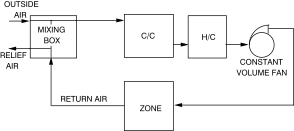
\includegraphics[width=0.9\textwidth, height=0.9\textheight, keepaspectratio=true]{media/image31.svg.png}
\caption{Simplified Single Zone Draw Through Air System \protect \label{fig:simplified-single-zone-draw-through-air}}
\end{figure}

The amount of heating or cooling provided by the air system in relation to the desired zone air temperature is given by:

\begin{equation}
{\dot Q_{sys}} = {\dot m_{sys}}{C_p}\eta \left( {{T_{\sup }} - {T_{z,\,desired}}} \right)
\end{equation}

where $\eta$ is the fraction of the time step that the air system is turned on and varies between 0 and 1. The supply air temperature is also implicitly limited by the effectiveness of the coils and the operating parameters of the central plant components. These interactions are discussed later.

A far more complex, though again simplified, air system is the variable air volume (VAV) system, shown in Figure~\ref{fig:simplified-variable-volume-air-system.}. Simplified Variable Volume Air System. In VAV systems, the supply air temperature, as well as the supply air volume, are continuous functions of zone air temperature. As shown in Figure~\ref{fig:idealized-variable-volume-system-operation.}. Idealized Variable Volume System Operation., when the zone air temperature is between T\(_{cl}\) and T\(_{cu}\), cooling is required and the air system varies the supply air flow rate while maintaining a constant supply air temperature. When the zone air temperature is between T\(_{hl}\) and T\(_{hu}\), heating is required and air is supplied at a constant minimum flow rate while the supply air temperature is varied.

\begin{figure}[hbtp] % fig 6
\centering
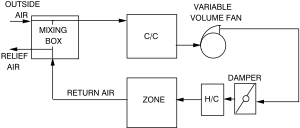
\includegraphics[width=0.9\textwidth, height=0.9\textheight, keepaspectratio=true]{media/image33.svg.png}
\caption{Simplified Variable Volume Air System. \protect \label{fig:simplified-variable-volume-air-system.}}
\end{figure}

The next figure (Idealized variable volume system operation) shows idealized behavior of a VAV system; in practice, the air flow rate and temperature are not exact linear functions of zone air temperature.

\begin{figure}[hbtp] % fig 7
\centering
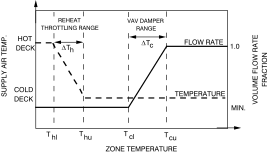
\includegraphics[width=0.9\textwidth, height=0.9\textheight, keepaspectratio=true]{media/image34.svg.png}
\caption{Idealized Variable Volume System Operation. \protect \label{fig:idealized-variable-volume-system-operation.}}
\end{figure}

As long as a VAV system has sufficient capacity, the zone air temperatures can be expected to vary within the limits defining the range of operation of the air damper, when cooling, or the throttling range of the reheat coil, when the air system is heating. This means that the desired zone air temperature, used to predict the air system response, is variable and must be calculated in order to determine the air system output. For the purposes of this calculation, the following definitions were found useful:

\begin{equation}
{\dot Q_0} = \sum\limits_{i = 1}^{{N_{sl}}} {{{\dot Q}_i}}  + \sum\limits_{i = 1}^{{N_{surfaces}}} {{h_i}} {A_i}{T_{si}} + \sum\limits_{i = 1}^{{N_{zones}}} {{{\dot m}_i}} {C_p}{T_{zi}} + {\dot m_{\inf }}{C_p}{T_\infty }
\label{eq:ZoneMeanAirTempUpdatingNumerator}
\end{equation}

\begin{equation}
{\dot Q_{slope}} = \sum\limits_{i = 1}^{{N_{surfaces}}} {{h_i}} {A_i} + \sum\limits_{i = 1}^{{N_{zones}}} {{{\dot m}_i}} {C_p} + {\dot m_{\inf }}{C_p}
\label{eq:ZoneMeanAirTempUpdatingDenominator}
\end{equation}

Equations~\ref{eq:ZoneMeanAirTempUpdatingNumerator} and~\ref{eq:ZoneMeanAirTempUpdatingDenominator} are derived, respectively, from the numerator and denominator of Equation~\ref{eq:ZoneTemperatureUpdateEquation} but with the system related terms omitted. Also excluded from these expressions are the effects of zone capacitance.

When a zone requires cooling, the VAV system is designed to provide air to that zone at a constant supply air temperature. The amount of cooling is matched to the load by dampers in the supply air duct that vary the air volume flow rate of being supplied to the zone. Assuming that the volume flow rate varies linearly with zone air temperature, the volume flow rate of supply air normalized to the maximum flow rate, or supply air fraction, is given by:

\begin{equation}
{\eta_c} = {\eta_{c,\,\min }} + \left( {1 - {\eta_{c,\,\min }}} \right)\left( {\frac{{{T_z} - {T_{c,\,lower}}}}{{{T_{c,\,upper}} - {T_{c,\,lower}}}}} \right);\,{\eta_{c,\,\min }} \le {\eta_c} \le 1.0
\label{eq:NormalizedSupplyAirFlowC}
\end{equation}

Normally, the minimum supply air fraction $\eta$\(_{c,min}\) must be greater than zero to ensure a supply of fresh air sufficient to eliminate contaminants from the zone.

Conversely, when heating is required in a zone, the VAV system becomes a constant volume flow rate system with a variable supply air temperature. The dampers are set to provide air to the zone at the minimum supply air fraction. Throttling the hot water supply to the reheat coil, which effectively alters the coil's heating capacity, modulates the supply air temperature. Again, assuming the heat energy output varies linearly with zone air temperature and normalizing with respect to the maximum coil output gives the following result:

\begin{equation}
{\eta_h} = \left( {\frac{{{T_{h,\,upper}} - {T_z}}}{{{T_{h,\,upper}} - {T_{h,\,lower}}}}} \right);\,0 \le {\eta_h} \le 1.0
\label{eq:NormalizedSupplyAirFlowH}
\end{equation}

Observe that when $\eta$\(_{h}\) is equal to zero, the zone is supplied with air at the cooling coil outlet temperature at the minimum air fraction. Because the control strategies of the VAV system are different whether the air system is heating or cooling, two equations are necessary to describe the air system output in terms of $\eta$\(_{h}\) and $\eta$\(_{c}\). These expressions are as shown in Equations~\ref{eq:AirSystemOutputH} and~\ref{eq:AirSystemOutputC}:

\begin{equation}
{\dot Q_{sys,h}} = {\eta_h}{\dot Q_{h/c,\,\max }} + {C_p}\rho {\dot V_{\min }}\left( {{T_{c/c}} - {T_{z,pred,heat}}} \right)
\label{eq:AirSystemOutputH}
\end{equation}

\begin{equation}
{\dot Q_{sys,c}} = {C_p}\rho \left( {{\eta_c}{{\dot V}_{\max }}} \right)\left( {{T_{c/c}} - {T_{z,pred,cool}}} \right)
\label{eq:AirSystemOutputC}
\end{equation}

Equation~\ref{eq:AirSystemOutputH} is valid for zone air temperatures below T\(_{h,upper}\), while Equation~\ref{eq:AirSystemOutputC} is valid for all temperatures above this value. Equating the system output to the zone load, as given by Equation~\ref{eq:NetZoneLoadEquation}, the definitions of $\eta$\(_{c}\) and $\eta$\(_{h}\) were then used to develop expressions for the predicted zone air temperature in the cases of heating and cooling:

\begin{equation}
{T_{z,pred,heat}} = \frac{{{{\dot Q}_{h/c,\max }}{T_{h,upper}}}}{{{T_{h,upper}} - {T_{h,lower}}}} + {\dot Q_0} + \frac{{{C_p}\rho {{\dot V}_{\min }}{T_{c/c}}}}{{\frac{{{{\dot Q}_{h/c,\max }}}}{{{T_{h,upper}} - {T_{h,lower}}}} + {C_p}\rho {{\dot V}_{\min }} + {{\dot Q}_{slope}}}}
\label{eq:PredictedZoneAirTempHeat}
\end{equation}

\begin{equation}
{T_{z,pred,cool}} = \frac{{{B_1} + \sqrt {B_1^2 + {B_2}} }}{2}
\label{eq:PredictedZoneAirTempCool}
\end{equation}

where,

\begin{equation}
{B_1} = {T_{c/c}} + {T_{c,lower}} - \frac{{{\eta_{c,\min }} - {C_2}}}{{{C_1}}}
\end{equation}

\begin{equation}
{B_2} = 4\left( {\frac{{{C_3}}}{{{C_1}}} + {T_{c/c}}\left( {\frac{{{\eta_{c,\min }}}}{{{C_1}}} - {T_{c,lower}}} \right)} \right)
\end{equation}

and,

\begin{equation}
{C_1} = \frac{{1 - {\eta_{c,\min }}}}{{{T_{c,upper}} - {T_{c,lower}}}}
\end{equation}

\begin{equation}
{C_2} = \frac{{{{\dot Q}_{slope}}}}{{{C_p}\rho {{\dot V}_{\max }}}}
\end{equation}

\begin{equation}
{C_3} = \frac{{{{\dot Q}_0}}}{{{C_p}\rho {{\dot V}_{\max }}}}
\end{equation}

Once the predicted zone air temperature has been calculated from Equations~\ref{eq:PredictedZoneAirTempHeat} and~\ref{eq:PredictedZoneAirTempCool}, the air system response may be determined. When a zone requires cooling, the system supply air temperature is constant at the cooling coil outlet temperature and the volume flow rate is given by:

\begin{equation}
{\dot V_{supply}} = {\eta_c}{\dot V_{max}}
\label{eq:VDotCCoilOutlet}
\end{equation}

where the supply air fraction $\eta$\(_{c}\) is computed from Equation~\ref{eq:NormalizedSupplyAirFlowC}. When heating is required by the zone, the air system provides air at the minimum volume flow rate and at a temperature given by:

\begin{equation}
{T_{supply}} = {T_{c/c}} + \frac{{{\eta_h}{{\dot Q}_{h/c,max}}}}{{{C_p}\rho {{\dot V}_{min}}}}
\label{eq:TempSupplyAtMinFlowRate}
\end{equation}

The reheat coil capacity fraction $\eta$\(_{h}\) is determined by using Equation~\ref{eq:NormalizedSupplyAirFlowH}. Once Equation~\ref{eq:VDotCCoilOutlet} or~\ref{eq:TempSupplyAtMinFlowRate} has been used, the supply air flow rate and temperature are known. These values are then used in Equation~\ref{eq:TztFromZoneAirEnergyBalance} to calculate the updated zone air temperature. The equations describing VAV system operation may be solved without iteration if the cooling coil outlet temperature is constant, i.e.~if the coil has infinite capacity, and if the reheat coil capacity varies linearly with zone air temperature. This is not the case, either in practice or in simulations, when realistic coil models are used. Therefore, an iteration scheme was developed that solved these equations simultaneously with the coil performance models.
